\chapter{Amazon Web Services}

\section{Introdução}
A Amazon Web Services (AWS) é uma plataforma de serviços em nuvem segura, oferecendo poder computacional, armazenamento de banco de dados, distribuição de conteúdo e outras funcionalidades para ajudar as empresas em seu dimensionamento e crescimento. Segundo pesquisas recentes \cite{rightscale}, é o provedor de nuvem que detém a maior parcela do mercado em termos de adoção, com aproximadamente 64\%. Sua gama de serviços é bastante ampla, como mostrado abaixo:

\begin{figure}[h!]
  \centering
  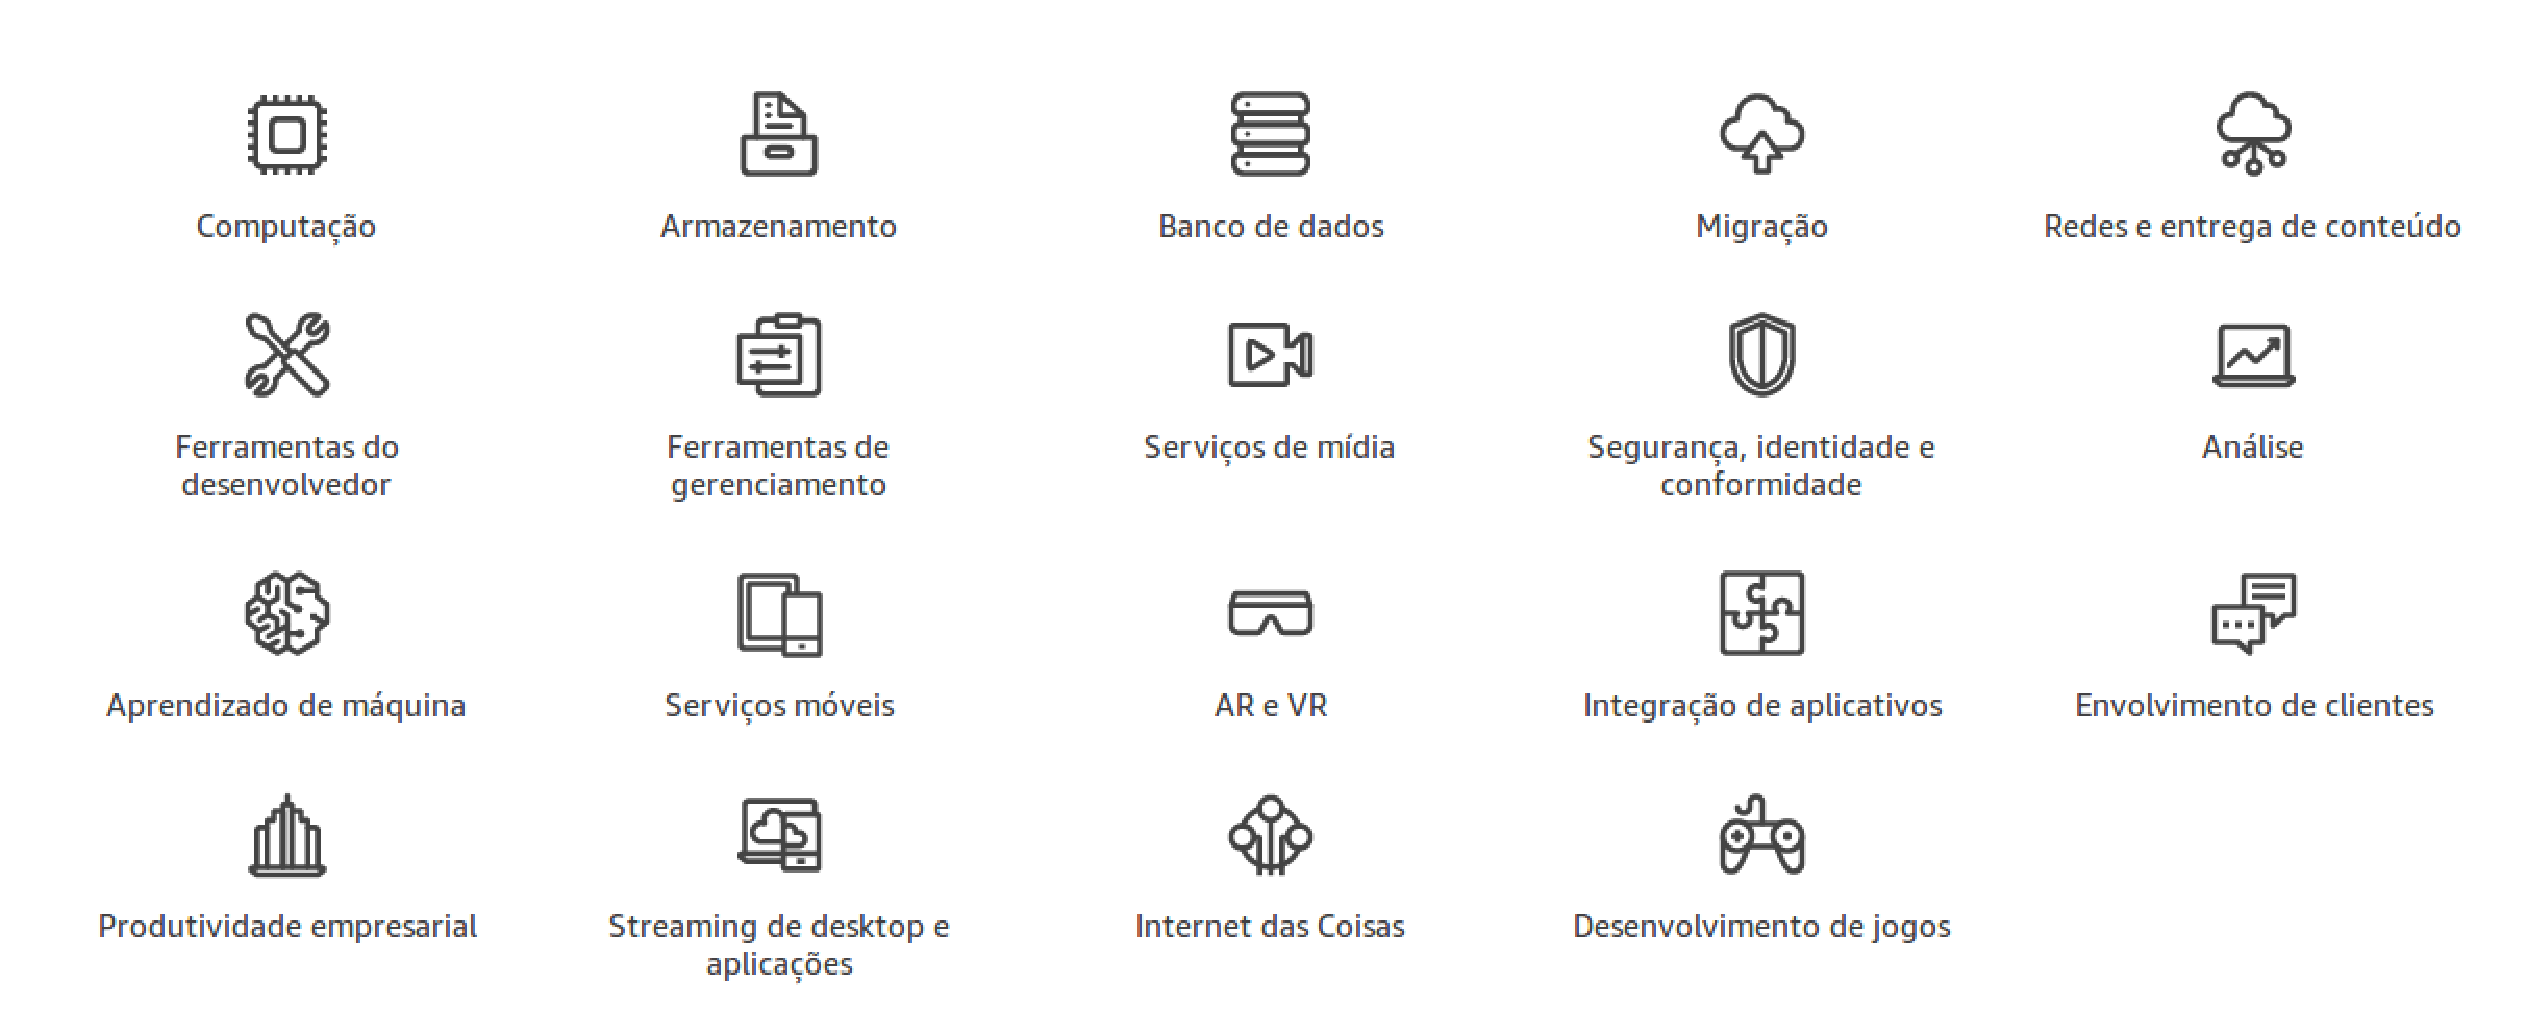
\includegraphics[scale=0.38]{imagens/aws-services.eps}
  \caption{Serviços da Amazon Web Services\cite{aws-services}}
\end{figure}

A AWS possui três serviços essenciais de nuvem para hospedagem de aplicações, sendo eles: \textbf{EC2}, \textbf{S3}, \textbf{RDS}. Além disso, possui soluções para outros variados campos da computação, como inteligência artificial, desenvolvimento \textit{mobile}, realidade virtual e internet das coisas.


\section{Funcionamento básico}
No contexto do documento, serão destacados os três serviços já citados anteriormente:


\begin{figure}[h!]
  \centering
  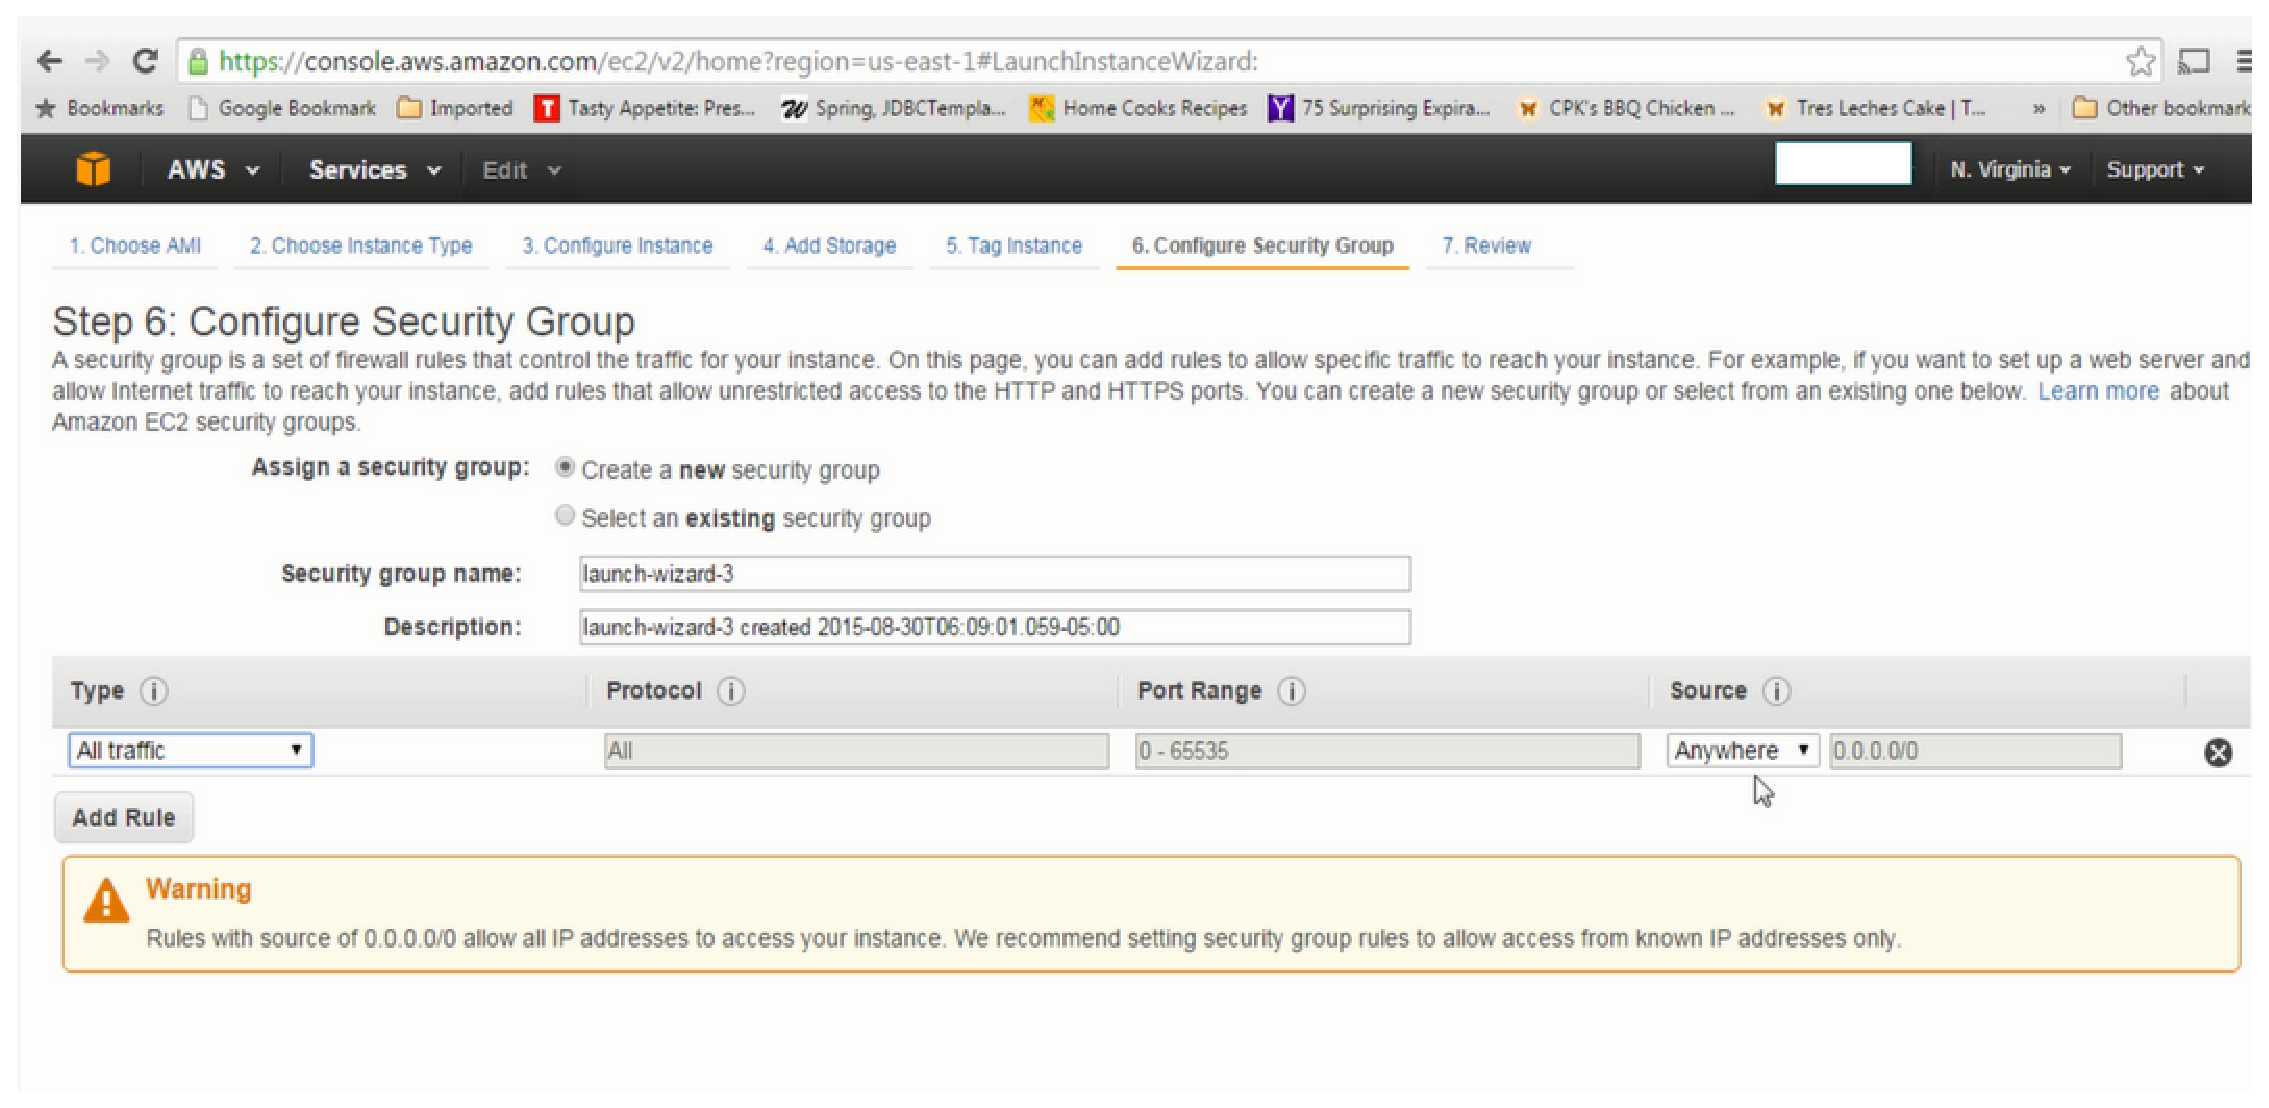
\includegraphics[scale=0.42]{imagens/aws-console.eps}
  \caption{Console da Amazon Web Services}
\end{figure}


\subsection{EC2}
O Amazon Elastic Compute Cloud (Amazon EC2) é o principal e mais básico serviço da AWS, e \textit{web} que disponibiliza capacidade computacional segura e redimensionável na nuvem. Ele foi criado para facilitar para os desenvolvedores a computação em nuvem na escala da \textit{web}. Possui várias \textit{features} bastante interessantes, com destaque para:
\begin{itemize}
  \item{\textbf{Elasticidade}: O Amazon EC2 permite aumento ou diminuição da capacidade em minutos em vez de horas ou dias. É possível contratar simultaneamente uma, centenas ou até milhares de instâncias de servidor. Também é possível usar o Amazon EC2 \textit{Auto Scaling} para manter a disponibilidade de frotas do EC2, além de ampliar e reduzir a escala dela, dependendo das necessidades específicas, com o objetivo de maximizar a performance e minimizar os custos;}
  \item{\textbf{Integração}: O serviço é integrado com uma séria de outros serviços da AWS, de maneira a prover um ambiente de computação em nuvem completo e seguro para uma série de possíveis aplicações do desenvolvedor;}
  \item{\textbf{Confiabilidade}: O EC2 oferece um ambiente altamente confiável, permitindo a contratação de instâncias de substituição de forma rápida e previsível. O serviço é executado dentro dos datacenters e da infraestrutura de rede comprovada da Amazon;}
  \item{\textbf{Baixo Custo}: Taxas são baixas e compatíveis com o poder computacional que realmente é utilizado pelo desenvolvedor.}
\end{itemize}

\subsection{S3}
O S3 (\textit{Simple Storage Service}) é o sistema de armazenamento da AWS. Segundo a definição da própria Amazon \cite{aws-s3}:

\begin{citacaoLonga}
Armazenamento de objetos para armazenar e recuperar qualquer quantidade de dados de qualquer local.
\end{citacaoLonga}

Possui bastante estabillidade e resiliência (compromisso de 99,999999999\% \cite{aws-s3}), visto que os dados são distribuídos automaticamente entre no mínimo três instalações físicas, separadas geograficamente dentro de uma região da AWS. Permite inclusive a replicação de dados entre as regiões da própria AWS.

É uma das soluções com maior porcentagem de adoção da Amazon, havendo inúmeros casos de sucesso de empresas grandes e com demandas bastante complexas. Cabe citar dois exemplos interessantes do mercado, e em áreas distintas: 
\begin{itemize}
  \item{\textit{\textbf{Netflix}}: empresa americana de \textit{streaming} de vídeo, disponibiliza bilhões de horas de conteúdo para clientes em todo o mundo atráves do S3. Além disso, usa o serviço como \textit{data lake} para suas soluções de \textit{big data}}.
  \item{\textit{\textbf{Airbnb}}: serviço online para que pessoas anunciem e reservem acomodações e meios de hospedagem. Utiliza o Amazon S3 para armazenar arquivos estatístcos e de \textit{backup}, além de mais de 10 Petabytes de fotografias de usuários e de acomodações.}
\end{itemize}

\subsection{RDS}

O Amazon RDS (\textit{Relational Database System}) é uma solução que fornece bancos de dados relacionais gerenciados, de maneira escalável e automatizando uma série de funções como administração, aplicação de \textit{patches} e \textit{backups}. Atualmente, trabalham com cinco dos principais mecanismos de bancos de dados SQL do mercado (tanto \textit{open source} como proprietários). São eles: 

\begin{itemize}
  \item{PostgreSQL}
  \item{MySQL}
  \item{MariaDB}
  \item{Oracle}
  \item{Microsoft SQL Server}
\end{itemize}

Além disso, possuem uma solução de banco de dados própria, o \textbf{Amazon Aurora}, que é compatível com o MariaDB e o PostgreSQL, e também roda nas instâncias do RDS. Conforme citado no próprio site da AWS \cite{aws-aurora}:

\begin{citacaoLonga}
O Aurora é até cinco vezes mais rápido que bancos de dados MySQL padrão e três vezes mais rápido que bancos de dados PostgreSQL padrão. O serviço oferece a segurança, a disponibilidade e a confiabilidade de bancos de dados comerciais por um décimo do custo.
\end{citacaoLonga}

\section{Outros Serviços}

Para representar a vasta gama de serviços em nuvem que a AWS apresenta, pode ser citada a \textbf{Amazon Alexa}, um serviço de voz e inteligência artificial que permite a construção de experências de voz naturais, promovendo um meio para que os clientes interajam com a tecnologia do dia a dia. A Alexa possui uma coleção bastante rica de ferramentas, \textit{APIs} e documentação que tornam seu desenvolvimento bem acessível.


\section{Conclusão}

A AWS não é a líder de mercado (em termos de adoção) de \textit{cloud computing} atoa. Apresenta soluções de qualidade em praticamente todos os campos da computação, desde áreas mais consolidads como hospedagem mais simples de aplicativos, como em campos mais de pesquisa como \textit{machine learning} e inteligência artificial. A única desvantagem que pode apresentar com relação aos seus concorrentes seria com relação ao custo dos serviços, porém acaba dependendo bastante do propósito e do \textit{budget} de cada empresa ou usuário.
